\documentclass{fithesis}

\usepackage{lmodern}
\usepackage[czech]{babel}
\usepackage[utf8]{inputenc}
\usepackage{cmap}
\usepackage{graphicx}
\usepackage[T1]{fontenc} %formátuje české znaky - důležité
\usepackage[plainpages=false, pdfpagelabels]{hyperref}
\usepackage{hyperref}
%\usepackage{makeidx}
%\makeindex

%\bibliographystyle{unsrt}


%\makeindex
\thesistitle{Integrace DMS a workflow v Liferay Portal}
\thesissubtitle{Diplomová práce}
\thesisstudent{Marek Tlačbaba}
\thesiswoman{false}
\thesisfaculty{fi}
\thesisyear{2014}
\thesisadvisor{RNDr. Jaroslav Ráček, Ph.D.}


\begin{document}

\FrontMatter
\ThesisTitlePage

\begin{ThesisDeclaration}
Prohlášení\AdvisorName
\end{ThesisDeclaration}

\begin{ThesisThanks}
Poděkování
\end{ThesisThanks}

\begin{ThesisAbstract}
Abstrak
\end{ThesisAbstract}

\begin{ThesisKeyWords}
Klíčová slova
\end{ThesisKeyWords}


\MainMatter
\setcounter{secnumdepth}{4}
\tableofcontents

\chapter{Úvod}
Oficiální zadání

Popsat principy tvorby podnikových portálů. Zaměřit se zejména na otázku implementace workflow pro procesy pracující s vnitropodnikovými dokomenty. Pro Liferay Portal verze CE analyzovat, navrhnout, implementovat, otestovat a zdokumentovat vlastní grafický workflow editor pracující v základní notaci BPMN, který bude plně kompatibilní se standardním workflow systémem, který je součástí Liferay Potral CE. Výstup bude mít podobu funkčního prototypu.

\chapter{Podnikové portály}

Pojem portál bývá definován různými způsoby v závislosti na situaci, ve které je používán. Dříve se portály zaměřovaly hlavně a jenom kolem jednotného přístupu k informacím nezávisle na jejich původu a umístění. S~dalším vývojem informačních technologií se postupně tento přístup dále rozšiřoval a~do definice portálu přibyly pojmy jako integrace a agregace služeb a aplikací. 

V následujícím textu je uvedno několik definic portálu a podnikového portálu.

\begin{itemize}

\item Například Gála definoval portál jako jednotné rohraní, ve kterém lze pracovat s běžnými službami a nástroji jako jsou, například zpravodajství a~komunikace, mimo to je v něm zaručen přístup k všeobecným aplikacím jako jsou vlastní stránky a blogy, a k aplikacím specializovaným, například slovníkům. \cite{gala}

\item Tato definice portálu je převzata ze standardu JSR-286 a zní následovně: Portál je webová aplikace, která (obvykle) poskytuje možnost personalizace, autentifikace, agregace obsahu z různých zdrojů a slouží jako prezentační vrstva informačních systémů. Agregací se rozumí integrace obsahu z různých zdrojů v rámci jedné webové stránky. Portál může mít vysoce propracované nástroje pro personalizaci, které poskytují obsah upravitelný podle přání uživatele. Stránky portálu mohou mít různé skupiny portletů \footnote[1]{Bližší informace v dalších částech této práce.}, které vytvářejí obsah pro různé uživatele.  \cite{jsr-286}

\item Předchozí defince se týkají portálu obecně, proto zde uvedu také definici podnikového portálu jako takového. Například podle Čecha je podnikový portál definován jako internetové nebo intranetové stránky, které slouží jako vstupní bod, respektive brána k různým datovým, informačním a znalostním zdrojům v organizaci. Jejich cílem je zpřístupnit tyto zdroje specifické skupině lidí. Může to být jak zákazníkům, tak také vlastním zaměstnacům nebo partnerům. \cite{cech}

\end{itemize}

V předchozích definicích portálu jsou naznačeny některé základní rysy podnikových portálů. Mezi základní vlastnosti můžeme považovat jediný přístupový bod, integrace, federace, přizpůsobivost, personalizace, kontrola přístupu a vyhledávání v podnikovém obsahu, tak jak jsou uvedeny v \cite{enterprise-portal} 

\section{Konkrétní portálová řešení}
Existuje a používá se celá řada konkrétních portálových řešení. Nejčastěji bývají implementovány v jazyce Java a podporují standardy JSR-168 a JSR-286 \footnote[2]{Bližší informace v dalších částech této práce} pro tvorbu portletů v jazyce Java. Existují také portály i pro jiné technologie, například pro platformu .NET je možné využít Microsoft SharePoint, ale nejvíce řešení existuje pro jazyk Java, kde mezi nejznámější patří IBM Websphere Portal, JBoss GateIn, Oracle WebCenter či Liferay Portal. Tyto portály již většinou obsahují velké množství již připravaných portletů, např. wiki, správa souborů, komunikace a další podobné.

V praktické části této práce bude vytvořen portlet pro tvorbu workflow pomocí grafického designeru v portálu Liferay.

\section{Liferay Portal}
Liferay portal je open-source podnikový portál založený na jazyce Java vyvíjený společností Liferay, Inc.. Podporuje specifikace JSR-168 a JSR-286 pro tvorbu portletů v jazyce Java. Liferay Portal je k dispozici ve dvou edicích, Community Edition a Enterprise Edition.

Community Edition je bezplatná verze portálu, která je volně dostupná ke stažení. Tato verze je ale bez oficiální podpory, ta je dostupná pouze prostřednictvím Liferay komunity. Druhá verze portálu, Liferay Portal Enterprise Edition je placená edice. U této verze je kladen velký důraz na stabilitu, bezpečnost a výkon. K této edici patří dlouhodobá podpora od společnosti Liferay, Inc. nebo jejích partenerů.

Ihned po instalaci portálu je k dispozici množství již předinstalovaných portletů. Je možné například ihned využívat wiki, fórům, kalendář, galerii obrázků. Liferay portál podporuje různé způsoby, jak jej lze upravovat či rozšiřovat. Pro změnu vzhledu můžeme využít témata či šablony, dále funkcionalitu portálu je možno rozšířit pomocí portletů, měnit vlastnoti portálu či portletů je umožněno díky tzv. hooks a větší a zásadnější změny přímo v jádru portálu se provádí pomocí pluginu Ext. \cite{developer-guide}

Mezi hlavní a důežité vlastnosti portálu Liferay bývají nejčastěji řazeny tyto: \cite{liferay-features}
\begin{itemize}
\item zabezpečené jednotné přihlášení,
\item nástroje pro správu workflow,
\item snadná instalce samotného portálu i nových aplikací a rozšíření,
\item od verze 6.1 CE GA2 umožňuje instalaci rozšíření a aplikcí z Liferay Marketplace,
\item obsahuje systém pro správu obsahu (Liferay CMS), který umožňuje oprávněným uživatelům vytvářet a spravovat obsah webu přímo z prohlížeče i bez znalosti programování,
\item vícejazyčné uživatelské rozhraní,
\item personalizace portálových stránek,
\item jednoduchá úpráva stránek způsobem táhni a pusť,
\item umožňuje dělit uživavatele do organizací, či do skupin uživatelů a podle těchto rolí zobrazovat různý obsah či aplikace,
\item automatické nahrávání souborů,
\item podpora pro různé platformy - různé aplikační servery, operační systémy a databáze,
\item podporuje různé metody integrace včetně SOAP, REST, RSS a také různá proprietární rozhraní.
\end{itemize}

To jsou některé z důvodů, proč se podnikový portál Liferay stal rožšířenou a oblíbenou platformou pro vývoj firemních webů a systému v jazyce Java.

\chapter{Vývoj portletů}
V této kapitole bude popsán vývoj portletů, které tvoří obsah portálů.

\section{Portlet}
Portlet je webová aplikace, která poskytuje uživatelům specifický obsah, typicky informaci nebo službu. Portlet je spravován portletovým kontejnerem, který zpracovává požadavky portletu a následně generuje dynamický obsah v podobě fragmentů v některým ze značkovacích jazyků -- HTML, XHTML, WML.  Tyto fragmenty jsou pak spojovány a dohromady vytváří portálovou stránku.

Portletový kontejner má tedy opovědnost za řízení životního cyklu jedntlivých portletů a je v něm také uloženo nastavení uživatele pro daný portlet. Ale jednotlivé části generované jednotlivými portlety slučuje dohromady na stránku portál. Portál a portletový kontejner mohou postaveny jako jedna komponenta ale mohou být také jako komponenty dvě. Na následujícím obrázku 3.1 je zobrazen průběh vytváření stránky v portálu tak, jak bylo již výše naznačeno.

\begin{figure}[htp]
\centering
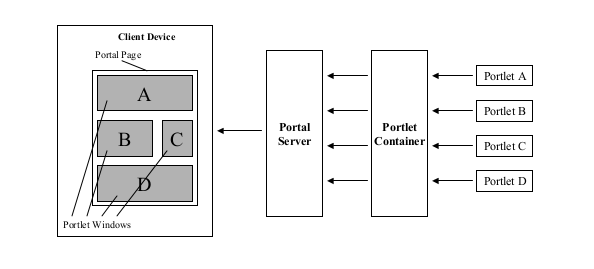
\includegraphics[width=340px]{images/vytvareni_stranky_v_portalu.png}
\caption{Vytváření stránky v portálu (převzato z \cite{jsr-286})}
\end{figure}

\section{Specifikace}
Důvodem pro vytvoření portletové specifikace byla situace, kdy různí dodavatelé používali svá vlastní API, která neumožňovala přenositelnost mezi portálovými servery.

První verze Java Portlet Specification 1.0 (JSR-168) byla vydána v roce 2003. V této specifikaci ještě bylo stále různé nedostatky a chyby, které pak tvůrci portletů stejně řešili každý po svém. To způsobovalo i nadále, že portlety byly mezi portálovými servery stále problematicky přenositelné či nepřenositelné úplně. Proto vznikla druhá verze Java Portlet Specification 2.0 (JSR-286) a ta byla vydána v červnu 2008. Mezi nejdůležitější přínosy patří následující:
\begin{itemize}
\item sdílení parametrů mezi portlety skrz veřejné render parametry,
\item meziportletová komunikace pomocí zasílaní událostí,
\item transformace informací nově definovanými portletovými filtry,
\item možnost portletů poskytovat zdroje jako jsou například PDF soubory.
\end{itemize}
Většina portletových kontejnerů sice poskytuje k základním požadavkům i svá rozšíření. Tyto rozšíření však nemusíme využívat a tak můžeme zachovat myšlenku snadné přenositelnosti.

\subsection{Životní cyklus portletu}
Každý portlet musí implementovat rozhraní \verb|Portlet|. Toto rozhraní obsahuje čtyři základní metody, které musí být implementovány a které řídí životní cyklus portletu - \verb|init(), processAction(), render(), destroy()|.

Metoda \verb|init()| je volána ihned při vytváření portletu a je používána například pro přípravu zdrojů potřebných portletem.



\chapter{Vzorová kapitola}
\section{Vzorová sekce}
\subsection{Vzorová podsekce}



\begin{itemize}
\item vzorový seznam
\end{itemize}


\begin{table}
\centering
\begin{tabular}{|p{3cm}|p{8cm}|}
\hline Sloupec 1 & Sloupec 2 \\
\hline Položka 2 & položka 2 \\
\hline
\end{tabular}
\caption{Vybrané skupinové adresy (převzato z \cite{satrapa-ipv6})}
\end{table}



%\printindex

\begin{thebibliography}{0}

\bibitem{gala}
GÁLA, L. et al. \textit{Podniková informatika}. 1. vyd. Praha: Grada Publishing, 2006. 

\bibitem{jsr-286}
\textit{JavaTM Portlet Specification}, The Java Community Process, dostupný na \url{http://www.jcp.org/en/jsr/detail?id=286} [cit. 2014-03-27].

\bibitem{cech}
ČECH, P. \textit {Přinos podnikových portálů pro management znalostí}, in Internet a konkurenceschopnost, Zlín, 2004.

\bibitem{enterprise-portal}
\textit{Enterprise portal}, Wikipedia, dostupný na \url{http://en.wikipedia.org/wiki/Enterprise_portal} [cit. 2014-03-27].

\bibitem{developer-guide}
\textit{Liferay Portal 6.2 Developer's Guide}, Liferay Inc., dostupný na \url{http://www.liferay.com/documentation/liferay-portal/6.2/development} [cit. 2014-04-02].

\bibitem{liferay-features}
\textit{Portal Features}, Liferay Inc., dostupný na \url{http://www.liferay.com/products/liferay-portal/features/portal} [cit. 2014-04-02].






\end{thebibliography}


\newpage
\appendix
\chapter{Položky seznamu}
asdfsadf

\chapter{Položky seznamu}
asdfsadf


\end{document}